\chapter{Variable Height CoM IS-MPC}
Before describing in detail the model \cite{SYROCO18} that allows humanoid 
robots to walk on uneven terrain (\textit{World of Stairs} in this case),
it is important to introduce the notation and 
to make an overview of the previous works.
Differently from manipulators, which are fixed to the ground, humanoids need 
to maintain equilibrium while walking. The contact with the ground is, in fact,
continuously changed due to walking itself. Usually, this is achieved by 
making sure that the ZMP (Zero Moment Point) is always within the convex hull 
of the support polygon. The ZMP, introduced in \cite{VUKOBRATOVIC19721}, is the 
point where the horizontal component of the moment of the ground reaction forces
becomes zero. To generate this kind of motion, usually a simplified model 
which only considers the CoM (center of mass) of the robot is used.
In particular, by neglecting the robot angular momentum and by assuming the 
CoM height is constant, the CoM dynamics can be treated as a LIP (Linear 
Inverted Pendulum), introduced for the first time in \cite{Kajita1991StudyOD}.
The Linear Inverted Pendulum model easily allows to design control schemes for 
the generation of the CoM reference trajectory, like the Preview Control 
\cite{Kajita2003BipedWP} and the Model Predictive Control
\cite{wieber:inria-00390462}.
Before discussing the LIP and extending it to the Variable Length Inverted
Pendulum, let's discuss the 3D motion model of the CoM reminding that the CoP
(Center of Pressure) in case of flat ground is the point of application of
the ground reaction force.

\section{3D Motion Model}
Let $(x_z, y_z, z_z)$ and $(x_c, y_c, z_c)$ respectively be the position of 
the ZMP and the position of the CoM. Assuming that the humanoid robot is walking 
on flat ground (hence the gravity acceleration components on $x$ and $y$ are 
zero) and neglecting the angular momentum around the CoM, the ZMP can be 
anywhere along the line connecting the CoP (located on the piece of surface 
upon which the support foot is placed) and the CoM (Fig. \ref{fig:lipm-robot}),
it is possible
\cite{kajita:intro-humanoid-robotics} to obtain the dynamics of the CoM:
\begin{align}
  \ddot{x}_c &= \frac{\ddot{z}_c + g}{z_c - z_z} (x_c - x_z) \\
  \ddot{y}_c &= \frac{\ddot{z}_c + g}{z_c - z_z} (y_c - y_z) \\
  \ddot{z}_c &= \frac{f_z}{m} - g
\end{align}
where $g$ is the gravity acceleration, $f_z$ is the z-component of the ground
reaction force, acting as an external input, and $m$ is the total mass of
the humanoid robot.
\begin{figure}
    \centering
    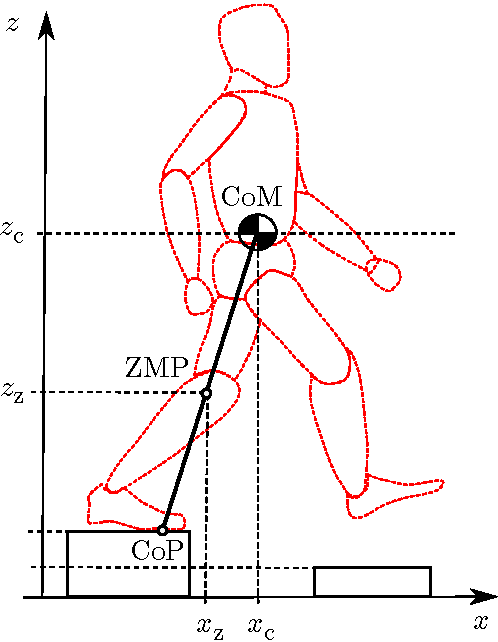
\includegraphics[width=0.5\textwidth]{figures/LIPM_robot.pdf}
    \caption{When walking on flat ground, or more in general on
        piecewise-horizontal ground as in the figure, the ZMP can be anywhere 
        between the line connecting the CoP and the CoM.}
    \label{fig:lipm-robot}
\end{figure}
The condition for maintaining equilibrium is that CoP is internal to the 
support polygon. Since the CoP, the CoM and the ZMP are colinear, as shown in 
Fig. \ref{fig:balance3d}, the condition is equivalent to the ZMP being internal
to the polyhedral cone having CoM as vertex and support
polygon as cross-section.
\begin{figure}
    \centering
    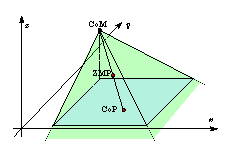
\includegraphics[width=0.7\textwidth]{figures/balance3d.pdf}
    \caption{The CoP should be internal to the support polygon, which is 
        equivalent to the ZMP being internal to the polyhedral cone with 
        the CoM as a vertex.}
    \label{fig:balance3d}
\end{figure}

\section{LIP}
The above motion model is nonlinear and difficult to use for gait generation.
Usually, to make the model linear, it is assumed that the ground is horizontal 
and the CoM has constant elevation with respect to the ground (i.e.
$z_c=\bar{z_c}$). As a consequence, it is possible to set $z_z=0$ making the 
CoP and the ZMP coincident, hence obtaining the LIP model:
\begin{align}
  \ddot{x}_c &= \omega_0^2 (x_c - x_z) \label{eq:lipm-x} \\
  \ddot{y}_c &= \omega_0^2 (y_c - y_z) \label{eq:lipm-y}
\end{align}
where $\omega_0^2 = g/\bar{z}_c$. This linear model, however, is not suitable 
for gait generation over uneven terrain.

\section{Variable Height CoM Motion Model}
Requiring the CoM to move at a constant height is not the only way to make the 
system linear. A more general way is to constraint its vertical motion such
that:
\begin{equation}
  \frac{\ddot{z}_c + g}{z_c - z_z} = \omega^2
\end{equation}
with $\omega$ arbitrary constant.

Using the above equation, the CoM dynamics become:
\begin{align}
  \ddot{x}_c &= \omega^2 (x_c - x_z) \label{eq:com-dynamics-x} \\
  \ddot{y}_c &= \omega^2 (y_c - y_z) \label{eq:com-dynamics-y}\\
  \ddot{z}_c &= \omega^2 (z_c - z_z) - g \label{eq:com-dynamics-z}
\end{align}
The above equations are linear and have a LIP-like structure with the 
ZMP coordinates $(x_z, y_z, z_z)$ acting as control inputs. This 3D model,
against the model of the LIP described in Eqs.
(\ref{eq:lipm-x}-\ref{eq:lipm-y}), allows vertical motion of the CoM, thus,
it can be used for 
gait generation on uneven terrain, considering the balance condition 
described by Fig. \ref{fig:balance3d}.

\section{MPC Formulation}
Before describing an MPC scheme for gait generation based on the above 
equations, it is important to notice that all of them include an unstable 
subsystem. For example, let's consider Eq. \eqref{eq:com-dynamics-x}. It is 
possible to decompose the system into a stable and an unstable subsystem by 
performing the following change of coordinates:
\begin{align}
  x_s = x_c - \dot{x}_c / \omega \\
  x_u = x_c + \dot{x}_c / \omega
\end{align}
The dynamics of $x_u$ is:
\begin{equation}
  \dot{x}_u = \dot{x}_c + \omega (x_c - x_z)
\end{equation}
which is unstable. It is however possible to prove 
\cite{Lanari2014BoundednessII} that $x_u$, and consequently $x_c$, will not 
diverge if a certain initial condition is satisfied (discussed in section 
\ref{sec:mpc-stability-constraint}). The same 
reasoning applies for the other two variables.

Let's perform a dynamic extension and choose the control variable as the ZMP 
velocities $\dot{x}_z, \dot{y}_z, \dot{z}_z$ rather than the ZMP itself. On the 
$x$ axis, the motion model becomes:
\begin{equation}
  \label{eq:vhcomlip-motion-model}
  \begin{pmatrix}
    \dot{x}_c \\
    \ddot{x}_c \\
    \dot{x}_z
  \end{pmatrix}
  =
  \begin{pmatrix}
    0 & 1 & 0 \\
    \omega^2 & 0 & -\omega^2 \\
    0 & 0 & 0
  \end{pmatrix}
  \begin{pmatrix}
    x_c \\
    \dot{x}_c \\
    x_z
  \end{pmatrix}
  +
  \begin{pmatrix}
    0 \\
    0 \\
    1
  \end{pmatrix}
  \dot{x}_z
\end{equation}
The same applies for the other two axes with an additive term $g$ appearing 
in the second equation of the dynamics along the $z$ axis.

Let's consider piecewise-constant control inputs over sampling intervals of
duration $\delta$, with a prediction horizon $T_h = N \cdot \delta$.
Let's denote the current time instant by $t_k$ and successive instants within
prediction horizon $t_{k+i}, i = 1, \dots, N$ by $t_{k+i}$.
At a generic instant $t_j$:
\begin{equation}
  \dot{x}_z(t) = \dot{x}_z^j, \quad t \in [t_j, t_{j+1})
\end{equation}
hence, the ZMP position along the $x$ axis in the time interval
$[t_j, t_{j+1}]$ is:
\begin{equation}
  x_z(t) = x_z^j + (t - t_j) \dot{x}_z^j, \quad t \in [t_j, t_{j+1}]
\end{equation}

\subsection{ZMP constraints}
Before describing the ZMP constraints in the 3D case (Fig. \ref{fig:balance3d}),
let's discuss the 2D case.

When walking on fully horizontal ground, the robot keeps the equilibrium 
if the ZMP remains inside the support polygon. Let's denote by
$(x_f^j, y_f^j, \theta_f^j)$ the pose of the 
generic footstep within the given sequence.
Let's use a fixed-shape moving ZMP constraint \cite{aboudonia17} to
enforce balance. The admissible region for ZMP at $t_{k+i}$ is centered in 
$(x_f^{k+i}, y_f^{k+i})$ and has orientation $\theta_f^{k+i}$.
In single support case, $(x_f^{k+i}, y_f^{k+i}, \theta_f^{k+i})$ coincide with
the pose of the support foot, hence, $(x_f^j, y_f^j, \theta_f^j)$.
In double support case, $(x_f^{k+i}, y_f^{k+i}, \theta_f^{k+i})$ gradually
slide from the position 
and orientation of the previous support foot to those of the next, as shown 
in Fig. \ref{fig:double-support}. 
\begin{figure}
    \centering
    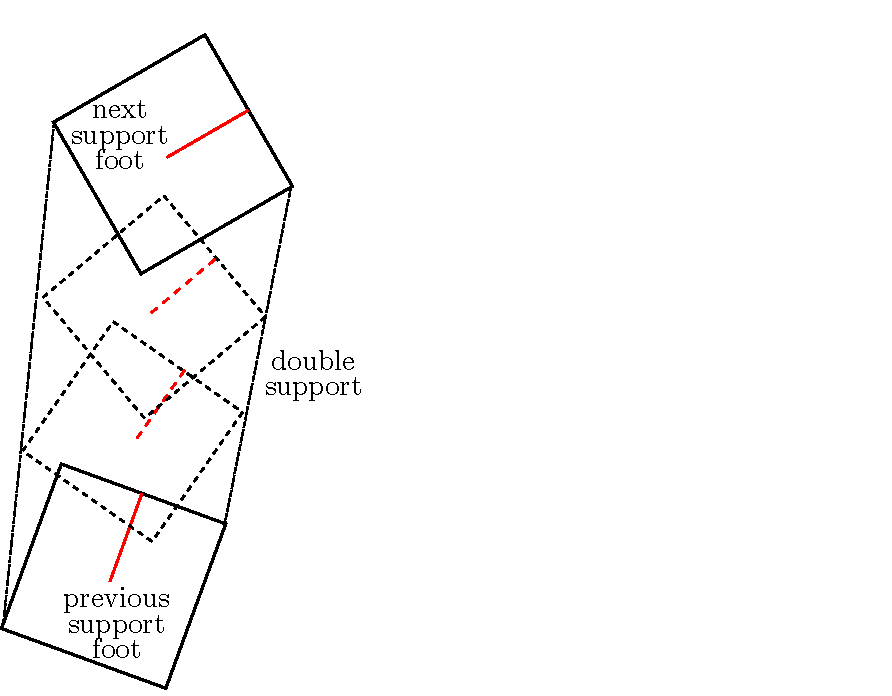
\includegraphics[width=0.3\textwidth]{figures/double_support.pdf}
    \caption{The ZMP constraint moves from a support foot to the following 
        one during double support phase.}
    \label{fig:double-support}
\end{figure}
The expression of the ZMP constraint in 2D can be written as:
\begin{equation}
  \label{eq:zmp-constraint-2d}
  -\frac{1}{2}
  \begin{pmatrix}
    d_x^\text{z} \\
    d_y^\text{z}
  \end{pmatrix}
  \le
  R_{k+i}^T
  \begin{pmatrix}
    x_z^{k+i} - x_f^{k+i} \\
    y_z^{k+i} - y_f^{k+i}
  \end{pmatrix}
  \le
  \frac{1}{2}
  \begin{pmatrix}
    d_x^\text{z} \\
    d_y^\text{z}
  \end{pmatrix}
\end{equation}
where $d_x^\text{z}$ and $d_y^\text{z}$ are the width and the height of the
rectangular constraint region and $R_{k+i}^T$ is the rotation matrix associated
to the orientation $\theta_f^{k+i}$.
Note that $(x_z^{k+i}, y_z^{k+i})$ is the predicted position
of the ZMP, which can be expressed as a linear combination of the control
variables:
\begin{equation}
  \label{eq:piecewise-linear-zmp-trajectory}
  x_z^{k+i} = x_z^k + \delta \sum_{i=0}^{i-1} \dot{x}_z^{k+j}
\end{equation}
Eq. \eqref{eq:zmp-constraint-2d} must be imposed for $i = 1, \dots, N$.

In the 3D case, the ZMP is allowed to leave the ground in order to
generate CoM motions along the $z$ axis as well.
As previously discussed, balance condition requires ZMP to remain inside
polyhedral cone defined by the support polygon and CoM
(Fig. \ref{fig:balance3d}. When ZMP is allowed to move vertically,
the constraint becomes nonlinear. In order to remove nonlinearity it is 
possible to consider a subregion of the polyhedral cone, for example a box
constraint, as shown in Fig. \ref{fig:polyhedral-cone-side-view}:
\begin{equation}
  \label{eq:zmp-constraint-3d}
  -\frac{1}{2}
  \begin{pmatrix}
    \tilde{d}_x^\text{z} \\
    \tilde{d}_y^\text{z} \\
    d_z^\text{z}
  \end{pmatrix}
  \le
  R_{k+i}^T
  \begin{pmatrix}
    x_z^{k+i} - x_f^{k+i} \\
    y_z^{k+i} - y_f^{k+i} \\
    z_z^{k+i} - y_f^{k+i}
  \end{pmatrix}
  \le
  \frac{1}{2}
  \begin{pmatrix}
    \tilde{d}_x^\text{z} \\
    \tilde{d}_y^\text{z} \\
    d_z^\text{z}
  \end{pmatrix}
\end{equation}
where $d_z^\text{z}$ defines the maximum allowed vertical ZMP displacement
with respect to the ground.
To guarantee that the box is contained in the cone, its $x$ and $y$ dimensions 
are respectively reduced to $\tilde{d}_x^\text{z}, \tilde{d}_y^\text{z}$:
\begin{equation}
  \tilde{d}_x^\text{z} = d_x^\text{z} \left( 1 -
      \frac{d_z^\text{z}}{2z_c^{\min}} \right)
      - \frac{d_z^\text{z}}{z_c^{\min}}\Delta x_c
\end{equation}
where $\Delta x_c$ is the maximum expected displacement of the CoM with respect 
to the center of the support foot and $z_c^{\min}$ is the minimum expected
value for CoM height. The same reasoning applies for $\tilde{d}_y^\text{z}$.
\begin{figure}
    \centering
    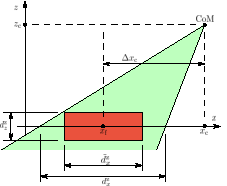
\includegraphics[width=0.7\textwidth]{figures/polyhedral-cone-side-view.pdf}
    \caption{The polyhedral cone representing the ZMP constraint and the 
        box used to approximate the constraint (which becomes linear).}
    \label{fig:polyhedral-cone-side-view}
\end{figure}
Similarly to the 2D case, the box constraint is kept fixed during
single support, while during double support the box 
slides linearly from its position around the previous support foot to its 
position around the next support foot, thus, always remaining within the 
polyhedral cone which defines the ZMP balance constraint, as shown in Fig.
\ref{fig:double-support3D}.
\begin{figure}
    \centering
    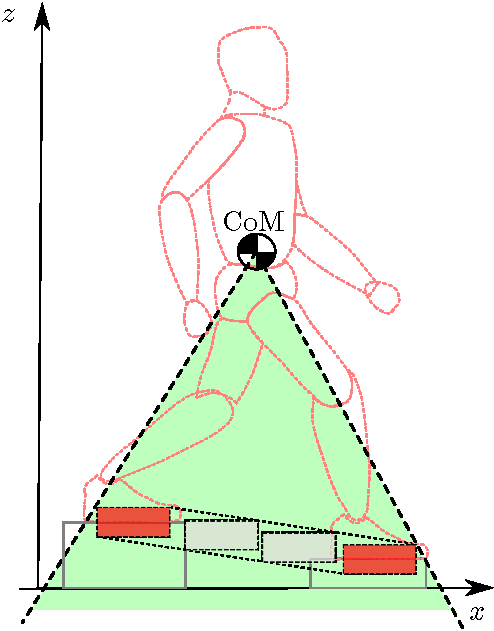
\includegraphics[width=0.5\textwidth]{figures/double_support3D.pdf}
    \caption{The ZMP box constraint moves from a support foot to the following 
        one during double support phase.}
    \label{fig:double-support3D}
\end{figure}
\subsection{Stability constraint}
\label{sec:mpc-stability-constraint}
As previously seen, the motion model
(\ref{eq:com-dynamics-x}-\ref{eq:com-dynamics-z}) is unstable, hence, it is 
not guaranteed that the CoM position is bounded with respect to the ZMP in 
general. This could make the generated gait unrealizable. However, as mentioned 
before and as discussed in \cite{Lanari2014BoundednessII,
DBLP:conf/humanoids/SciancaCSLO16}, it is possible to prove that if the 
initial condition $(x_c^k, \dot{x}_c^k)$ satisfies:
\begin{equation}
  \label{eq:stability-condition-xc}
  x_c^k + \frac{\dot{x}_c^k}{\omega} = \omega \int_{t_k}^\infty 
      e^{-\omega(\tau-t_k)}x_z(\tau)d\tau
\end{equation}
then $x_c$ remains bounded with respect to $x_z$ for
all $t$. An analogous condition can be given for $y_c$ dynamics.
Regarding $z_c$, it is possible to prove its boundedness by using the following
initial condition:
\begin{equation}
  \label{eq:stability-condition-zc}
  z_c^k + \frac{\dot{z}_c^k}{\omega} = \frac{g}{\omega^2} +
      \omega \int_{t_k}^\infty e^{-\omega(\tau-t_k)}z_z(\tau)d\tau
\end{equation}
The above stability conditions can be enforced in the MPC formulation by 
writing them with respect to the control variables $\dot{x}_\text{z}^{k+i},
\dot{y}_\text{z}^{k+i}, \dot{z}_\text{z}^{k+i}$. For $x_c$,
and similarly for $y_c$, the initial condition can be 
writtes as:
\begin{equation}
  \label{eq:stability-constraint-xdot}
  \frac{1}{\omega}\frac{1-e^{-\delta\omega}}{1-e^{-N\delta\omega}}
    \sum_{i=0}^{N-1} e^{-i\delta\omega} \dot{x}_z^{k+i} =
    x_c^k + \frac{\dot{x}_c^k}{\omega} - x_z^k
\end{equation}
which can be obtained from \eqref{eq:stability-condition-xc} by considering 
that the ZMP trajectory \eqref{eq:piecewise-linear-zmp-trajectory} is piecewise 
linear and that the contribution beyond the prediction horizon is computed 
assuming infinite replication of the control variables within the prediction 
horizon itself. A similar initial condition can be written for $z_c$
starting from \eqref{eq:stability-condition-zc}, where $\dot{z}_z$ is set to zero 
beyond the prediction horizon (truncated tail):
\begin{equation}
  \label{eq:stability-constraint-zdot}
  \frac{1-e^{-\delta\omega}}{1-e^{-N\delta\omega}}
    \sum_{i=0}^{N-1} e^{-i\delta\omega} \dot{z}_z^{k+i} =
    z_c^k + \frac{\dot{z}_c^k}{\omega} - z_z^k - \frac{g}{\omega^2}
\end{equation}
A more detailed discussion can be found in
\cite{DBLP:journals/corr/abs-1901-08505}.

\section{MPC Algorithm}
Now that the constraints have been expressed with respect to the input
variables, it is possible to define the MPC scheme used to generate the gait.
In particular, the MPC algorithm solves a QP problem at each iteration
determining the trajectory of the CoM. Note that the footsteps are assigned in 
advance.

Considering the decision variable vectors:
\begin{align}
  \dot{X}_\text{z}^k&=(\dot{x}_\text{z}^k, \dots, \dot{x}_\text{z}^{k+N-1})^T \\
  \dot{Y}_\text{z}^k&=(\dot{y}_\text{z}^k, \dots, \dot{y}_\text{z}^{k+N-1})^T \\
  \dot{Z}_\text{z}^k&=(\dot{z}_\text{z}^k, \dots, \dot{z}_\text{z}^{k+N-1})^T
\end{align}
the QP problem can be defined as:
\begin{align*}
  \min_{\dot{X}_\text{z}^k, \dot{Y}_\text{z}^k, \dot{Z}_\text{z}^k}
      &\sum_{i=1}^N
      \biggl[
          (\dot{x}_z^{k+i})^2 +
          (\dot{y}_z^{k+i})^2 +
          (\dot{z}_z^{k+i})^2 + \\
          &\beta \biggl(
              (x_z^{k+i} - x_f^{k+i})^2 +
              (y_z^{k+i} - y_f^{k+i})^2 +
              (z_z^{k+i} - z_f^{k+i})^2
          \biggr)
      \biggr]\\
      \textrm{s.t. } &\textrm{ZMP constraint \eqref{eq:zmp-constraint-3d}} \\
      &\textrm{stability constraints \eqref{eq:stability-constraint-xdot},
          \eqref{eq:stability-constraint-zdot}}
\end{align*}
where the cost function includes the decision variables for regularization 
purposes and a term which attempts to bring the ZMP to the center of the 
footstep.

Each MPC iteration starts at $t_k$ and executes the steps described in Algorithm
\ref{algo:mpc-iteration}, defining the trajectory of the CoM.
\begin{algorithm}
\SetAlgoLined
\KwResult{CoM trajectory}
  Compute $\dot{X}_\text{z}^k$, $\dot{Y}_\text{z}^k$, $\dot{Z}_\text{z}^k$ 
      that solve the QP problem\;
  From the solutions, extract the first control samples
      $\dot{x}_\text{z}^k$, $\dot{y}_\text{z}^k$, $\dot{z}_\text{z}^k$\;
  Set $\dot{x}_z=\dot{x}_\text{z}^k$ in \eqref{eq:vhcomlip-motion-model}
      and integrate from $(x_c^k, \dot{x}_c^k, x_\text{z}^k)$ to obtain 
      $x_c(t)$, $\dot{x}_c(t)$, $x_\text{z}(t)$ for
      $t \in [t_k, t_{k+1}]$. The same applies for for $y$, $z$.
  \caption{MPC iteration}
  \label{algo:mpc-iteration}
\end{algorithm}

\section{BHuman implementation}
The MPC scheme has been implemented in C++ upon the BHuman framework
\cite{BHumanCodeRelease2018} and it has been tested on both dynamic environments 
and NAO humanoid robot. The QP problem has been solved using qpOASES
\cite{qpOASES}. The footstep plan is either generated by the footstep planner 
described in Chapter \ref{ch:rrt-based-footstep-planning} or manually assigned 
before the execution of the program. Experiments are described in detail in 
Chapter \ref{ch:experiments}. Note that to speed up the execution of the code 
in order to keep computation within the sampling time of the kinematic 
controller, the rotation matrix of the ZMP constraint described in Eq.
\eqref{eq:zmp-constraint-3d} has been neglected. This does not create any
problem if the size of the box is small enough to stay within the poyhedral 
cone regardless of the rotation of the feet.

